% ============================================================================
% CHAPITRE 2 — LANCEMENT DU PROJET
% ============================================================================

\section{Introduction}

Ce chapitre est consacré au lancement du projet Guidni. Il vise à poser les bases nécessaires
avant d'entamer le développement itératif par Sprints. Pour cela, j'ai suivi le plan suivant~:
\begin{enumerate}
    \item Analyse et spécification des besoins fonctionnels et non fonctionnels
    \item Définitions théoriques des concepts clés
    \item Architecture fonctionnelle et logique
    \item Product Backlog
    \item Planification des Sprints
    \item Environnement de travail et outils
\end{enumerate}


% ────────────────────────────────────────────────────────────────
\section{Analyse des besoins}
% ────────────────────────────────────────────────────────────────

\subsection{Identification des acteurs}

Le système Guidni fait intervenir trois acteurs principaux~:

\begin{itemize}
    \item Le \textbf{Touriste}~: acteur principal qui interagit avec l'interface de chat pour
    formuler des demandes de planification, recevoir des itinéraires, et consulter des
    recommandations. Son comportement de navigation est automatiquement capté par le tracker
    JavaScript pour alimenter le moteur de recommandation.

    \item L'\textbf{Administrateur}~: responsable de la supervision technique. Il peut
    déclencher une reconstruction de l'index RAG, consulter l'état de santé du système et
    configurer le fournisseur LLM par défaut.

    \item Le \textbf{Système}~: ensemble des processus automatisés (écouteurs SQLAlchemy,
    tracker JavaScript, jobs nocturnes APScheduler, persistance des matrices LinUCB).
\end{itemize}

\subsection{Besoins fonctionnels}

Les besoins fonctionnels du système sont les suivants~:
\begin{itemize}
    \item \textbf{BF-01}~: Formuler des requêtes en langage naturel multilingue (FR/EN/AR)
    \item \textbf{BF-02}~: Générer des itinéraires multi-jours personnalisés (1 à 14~jours)
    \item \textbf{BF-03}~: Modifier un plan existant par des messages de suivi conversationnels
    \item \textbf{BF-04}~: Effectuer des recherches sémantiques dans le catalogue touristique
    \item \textbf{BF-05}~: Intégrer les données météorologiques en temps réel (Open-Meteo)
    \item \textbf{BF-06}~: Calculer les distances entre les sites (Haversine / Nominatim)
    \item \textbf{BF-07}~: Afficher des recommandations personnalisées en temps réel
    \item \textbf{BF-08}~: Collecter les signaux comportementaux du touriste
    \item \textbf{BF-09}~: Apprendre en ligne à partir des récompenses utilisateur
    \item \textbf{BF-10}~: Consulter et archiver l'historique des conversations
\end{itemize}

\subsection{Besoins non fonctionnels}

\begin{table}[H]
    \centering
    \caption{Besoins non fonctionnels du système Guidni}
    \label{tab:bnf}
    \small
    \begin{tabular}{p{2.8cm} p{5cm} p{5cm}}
        \toprule
        \textbf{Catégorie} & \textbf{Besoin} & \textbf{Cible} \\
        \midrule
        Performance & Latence endpoint \texttt{/chat} & $< 5$\,s (P95) \\
         & Latence recommandation & $< 100$\,ms (P95) \\[3pt]
        Disponibilité & Uptime du service & 99,5\% \\[3pt]
        Sécurité & Validation utilisateur & Vérification \texttt{user\_id} par requête \\
         & Limitation de débit & 10 événements/annonce/session \\[3pt]
        Multilingue & Langues supportées & FR, EN, AR (auto-détection) \\[3pt]
        Confidentialité & Données vers LLM & Pas de PII sans consentement \\
         & Option locale & Ollama pour souveraineté complète \\
        \bottomrule
    \end{tabular}
\end{table}

\subsection{Diagramme des cas d'utilisation global}

Le diagramme suivant présente une vue d'ensemble des interactions entre les trois acteurs
et les fonctionnalités principales du système.

\begin{figure}[H]
    \centering
    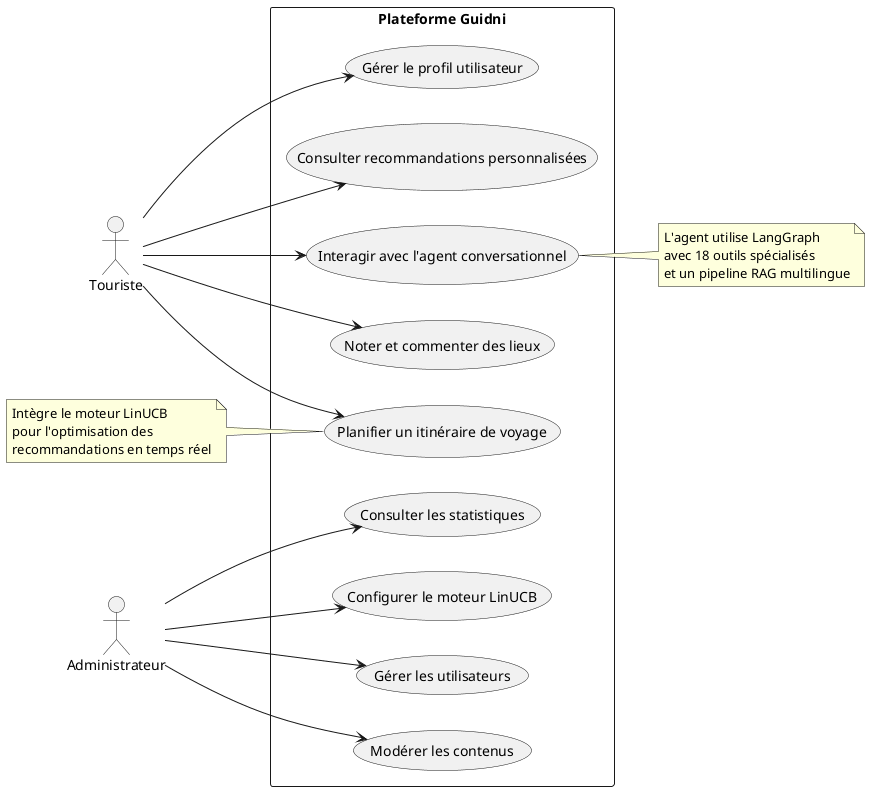
\includegraphics[width=\textwidth]{diagrams/plantuml/usecase_global.png}
    \caption{Diagramme de cas d'utilisation global du système Guidni}
    \label{fig:use_case_global}
\end{figure}


% ────────────────────────────────────────────────────────────────
\section{Définitions théoriques}
% ────────────────────────────────────────────────────────────────

Cette section présente les concepts théoriques fondamentaux sur lesquels repose le système
Guidni. Chaque concept est défini puis illustré par son application concrète dans le projet.

\subsection{Grands modèles de langage (LLM)}

L'architecture Transformer, introduite par Vaswani et al.~\cite{vaswani2017attention},
constitue le socle de tous les LLMs modernes. Son mécanisme d'attention multi-têtes permet de
pondérer l'importance relative de chaque token. L'ajustement par instructions et le RLHF
transforment un modèle de prédiction de tokens en un assistant capable d'exécuter des
instructions en langage naturel. L'appel d'outils (\textit{function calling}) permet au LLM
d'émettre un objet JSON structuré décrivant une fonction externe à appeler, plutôt que de
générer la réponse depuis sa mémoire paramétrique.

\begin{figure}[H]
    \centering
    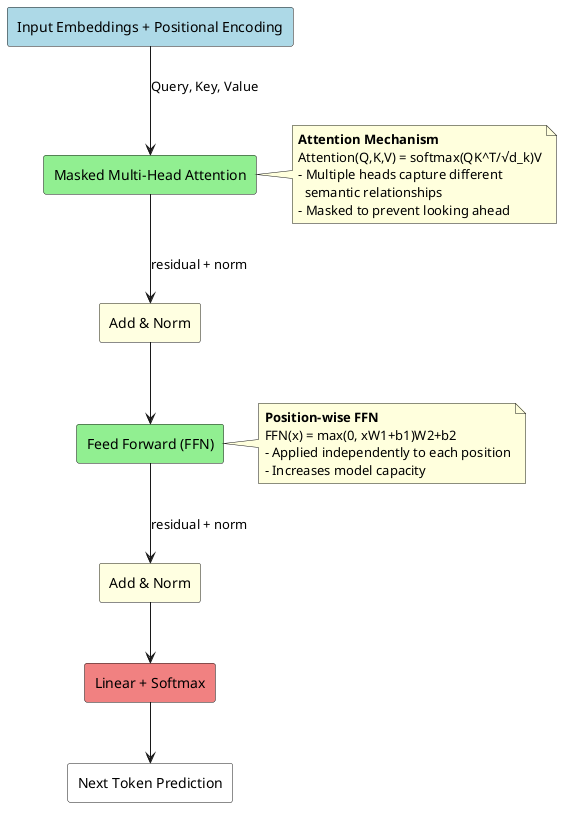
\includegraphics[width=0.75\textwidth]{diagrams/fig_02_transformer_attention.png}
    \caption{Architecture du Transformer avec mécanisme d'attention multi-têtes}
    \label{fig:transformer_arch}
\end{figure}

\subsection{Framework agentique LangGraph}

LangGraph, développé par LangChain Inc., étend le patron ReAct (\textit{Reason + Act})
proposé par Yao et al.~\cite{yao2023react} avec une machine à états typée explicite.
L'état de l'agent est défini par un \texttt{TypedDict} Python (\texttt{AgentState}) qui
accumule les messages, profils, données géolocalisées, compteurs de sécurité et indicateurs
décisionnels. Des fonctions de routage conditionnel déterminent quel nœud s'exécute ensuite.

Le graphe Guidni comporte quatre nœuds~: \textbf{THINK} (raisonnement du LLM),
\textbf{EXECUTE\_TOOL} (exécution d'un outil), \textbf{VALIDATE} (vérification du plan)
et \textbf{RESPOND} (formulation de la réponse). Une sortie forcée à 15~itérations empêche
les boucles infinies.

\begin{figure}[H]
    \centering
    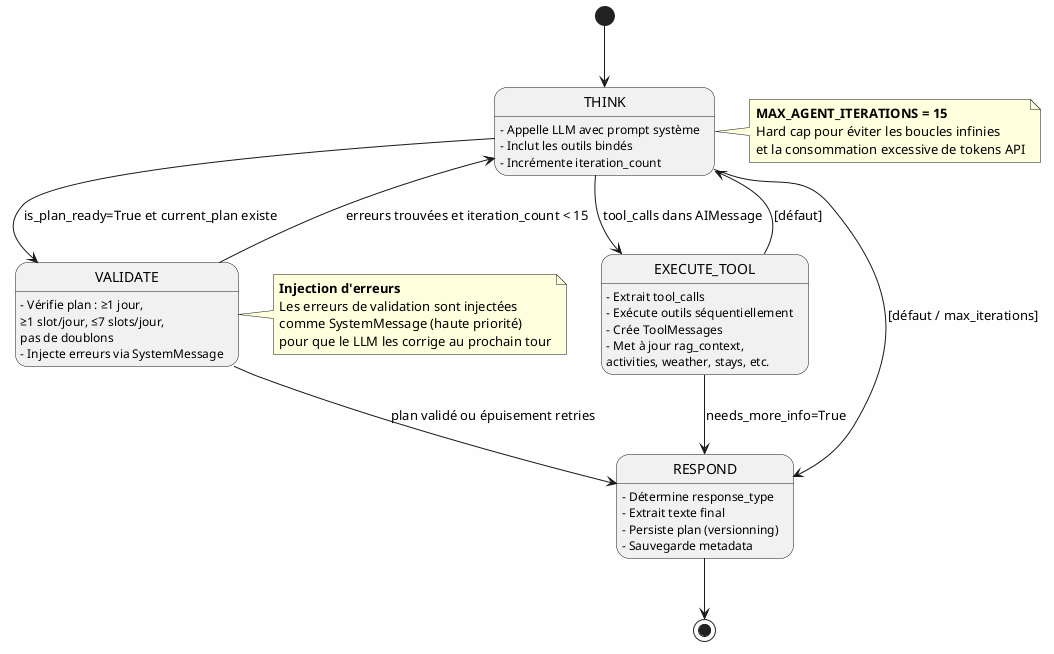
\includegraphics[width=0.7\textwidth]{diagrams/fig_02_langgraph_graph.png}
    \caption{Architecture LangGraph --- graphe d'états cyclique de l'agent}
    \label{fig:langgraph_arch}
\end{figure}

\subsection{Génération augmentée par récupération (RAG)}

Le principe RAG, formalisé par Lewis et al.~\cite{lewis2020rag}, consiste à récupérer des
documents pertinents depuis une base de connaissances et les injecter dans le prompt du LLM.
Le pipeline Guidni utilise BAAI/bge-m3 (embeddings multilingues 1024~dimensions, 100+~langues)
en première étape de récupération, suivi de bge-reranker-v2-m3 (cross-encoder) pour le
réordonnancement. L'index est maintenu à jour par réindexation incrémentale via les événements
SQLAlchemy (\texttt{after\_insert}, \texttt{after\_update}, \texttt{after\_delete}).

\begin{figure}[H]
    \centering
    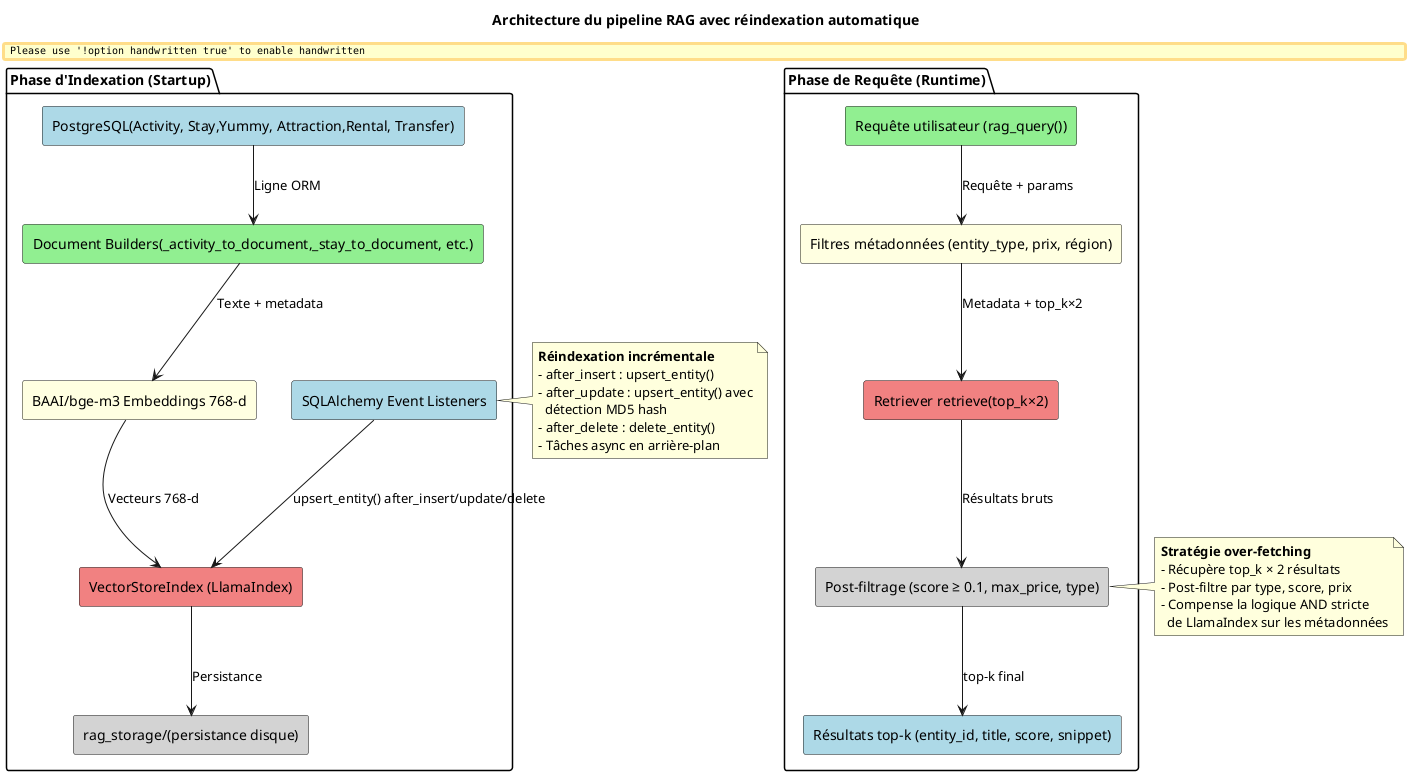
\includegraphics[width=0.85\textwidth]{diagrams/fig_02_rag_architecture.png}
    \caption{Architecture du pipeline RAG multilingue}
    \label{fig:rag_arch}
\end{figure}

\subsection{Bandits contextuels et algorithme LinUCB}

L'algorithme LinUCB~\cite{li2010linucb} suppose que la récompense espérée est une fonction
linéaire du vecteur de contexte~: $\mathbb{E}[r|\phi] = \theta^\top \phi$. Le score UCB
combine exploitation et exploration~:
\begin{equation}
    \text{score} = \underbrace{\hat{\theta}^\top \phi}_{\text{exploitation}} +
    \underbrace{\alpha \sqrt{\phi^\top A^{-1} \phi}}_{\text{exploration}}
    \label{eq:ucb_score}
\end{equation}

Le vecteur $\phi$ de dimension~306 est construit par produit de Kronecker~:
$\phi = x_{\text{user}}(9) \otimes x_{\text{tags}}(34)$, combinant le contexte utilisateur
(heure, mois, défilement, budget, type de voyage) avec les tags binaires des annonces.

\begin{figure}[H]
    \centering
    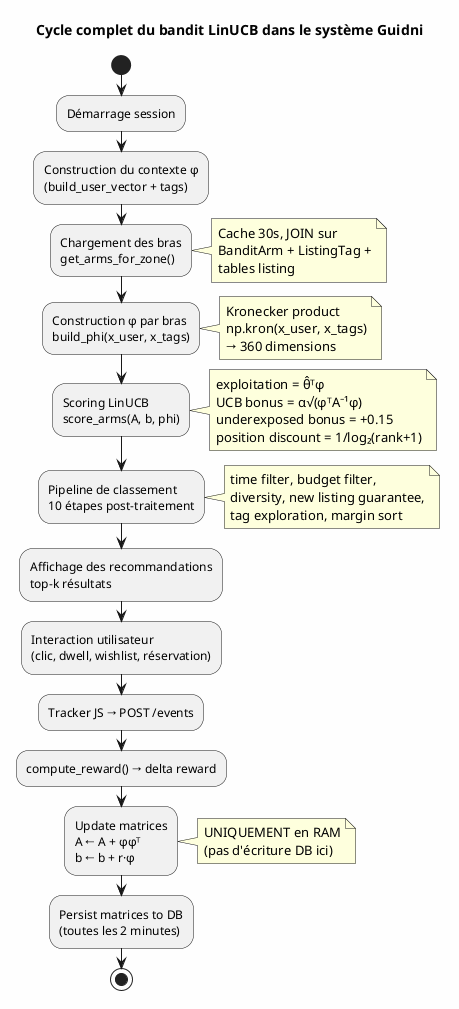
\includegraphics[width=0.7\textwidth]{diagrams/fig_02_linucb_cycle.png}
    \caption{Cycle exploitation / exploration du LinUCB}
    \label{fig:linucb_cycle}
\end{figure}

\begin{table}[H]
    \centering
    \caption{Étude comparative des approches de recommandation}
    \label{tab:reco_approaches}
    \small
    \begin{tabular}{p{3cm} p{2cm} p{2cm} p{2.5cm} p{2cm}}
        \toprule
        \textbf{Approche} & \textbf{Cold Start} & \textbf{Dérive} &
        \textbf{Données} & \textbf{Guidni~?} \\
        \midrule
        Filtrage collaboratif & Problématique & Mauvaise & Grand historique & Non \\[3pt]
        Basé contenu & Acceptable & Mauvaise & Attributs items & Partiel \\[3pt]
        Hybride offline & Partiel & Mauvaise & Les deux & Non \\[3pt]
        LinUCB contextuel & Bonus exploration & Reset $\lambda$-decay & Contexte TR & \textbf{Oui} \\
        \bottomrule
    \end{tabular}
\end{table}


% ────────────────────────────────────────────────────────────────
\section{Architecture fonctionnelle et logique}
% ────────────────────────────────────────────────────────────────

\subsection{Architecture fonctionnelle}

Le système Guidni repose sur l'articulation de deux sous-systèmes partageant une base de
données PostgreSQL 15 unifiée~:

\begin{itemize}
    \item Le \textbf{frontend} Next.js / Prisma gère l'interface utilisateur et les opérations
    CRUD sur les entités touristiques.
    \item Le \textbf{backend IA} FastAPI héberge l'agent planificateur LangGraph
    (9~endpoints REST) et le moteur de recommandation LinUCB (3~endpoints REST).
\end{itemize}

\begin{figure}[H]
    \centering
    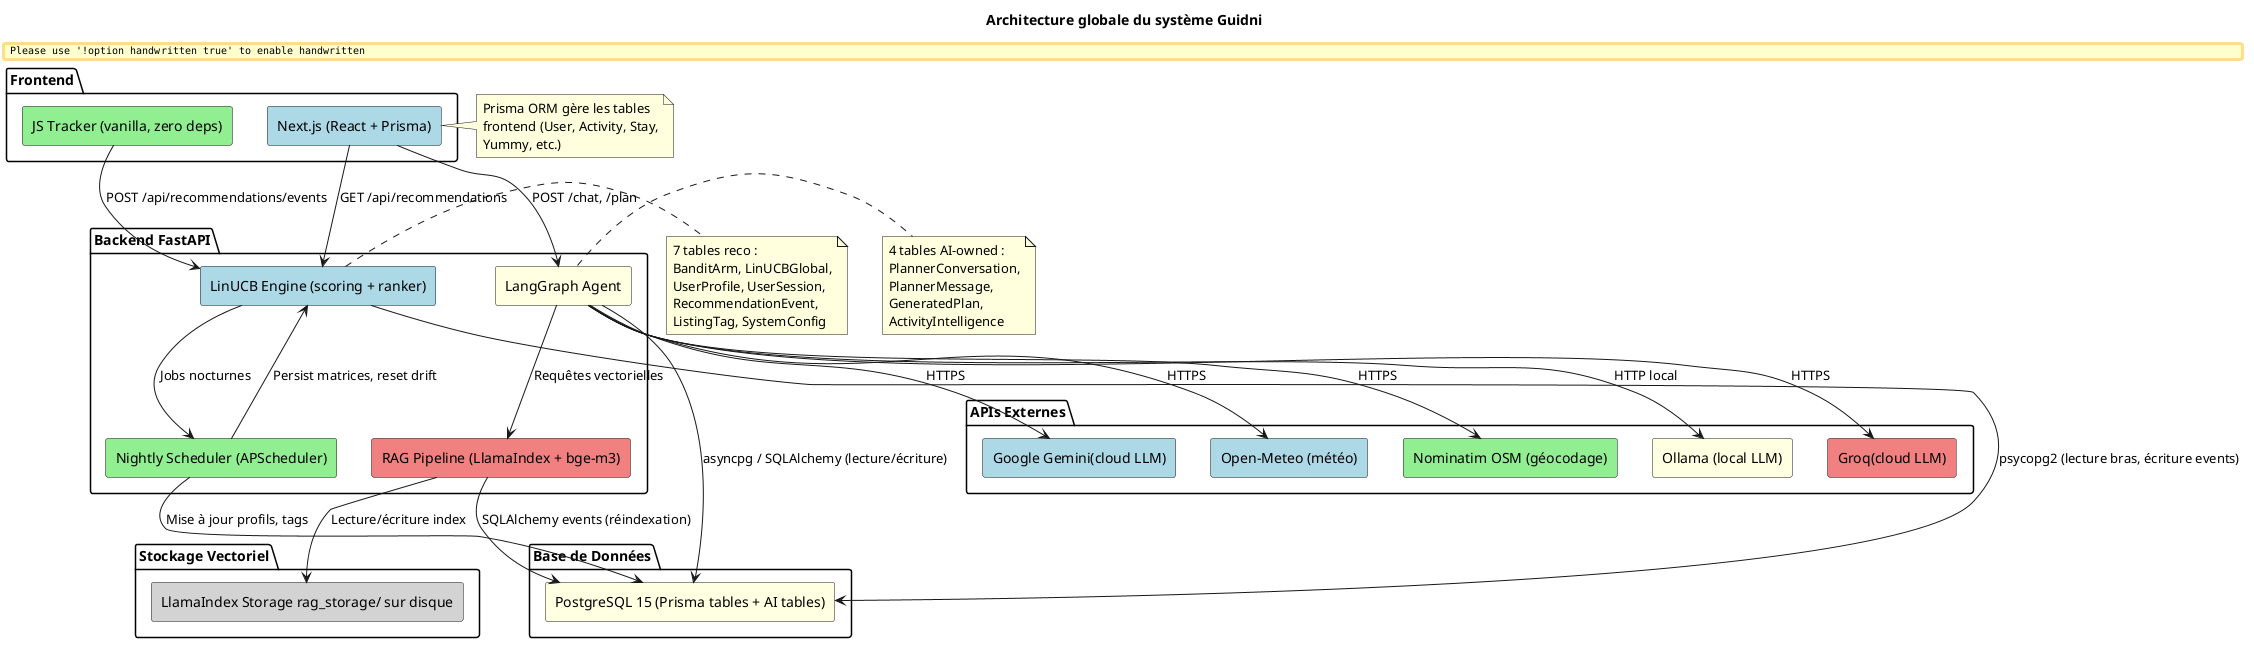
\includegraphics[width=\textwidth]{diagrams/fig_03_global_architecture.png}
    \caption{Architecture fonctionnelle du système Guidni}
    \label{fig:global_arch}
\end{figure}

\subsection{Architecture logique en couches}

L'architecture est organisée en quatre couches~:
\begin{enumerate}
    \item \textbf{Couche de présentation}~: endpoints FastAPI, schémas Pydantic, middleware CORS
    \item \textbf{Couche de logique métier}~: agent LangGraph (4~nœuds, 18~outils), moteur
    LinUCB (pipeline 10~étapes), moteur de requête RAG
    \item \textbf{Couche d'accès aux données}~: modèles SQLAlchemy, index LlamaIndex, pool
    psycopg2
    \item \textbf{Couche d'infrastructure}~: moteur AsyncPG, APScheduler, journalisation
    rotative
\end{enumerate}

\begin{figure}[H]
    \centering
    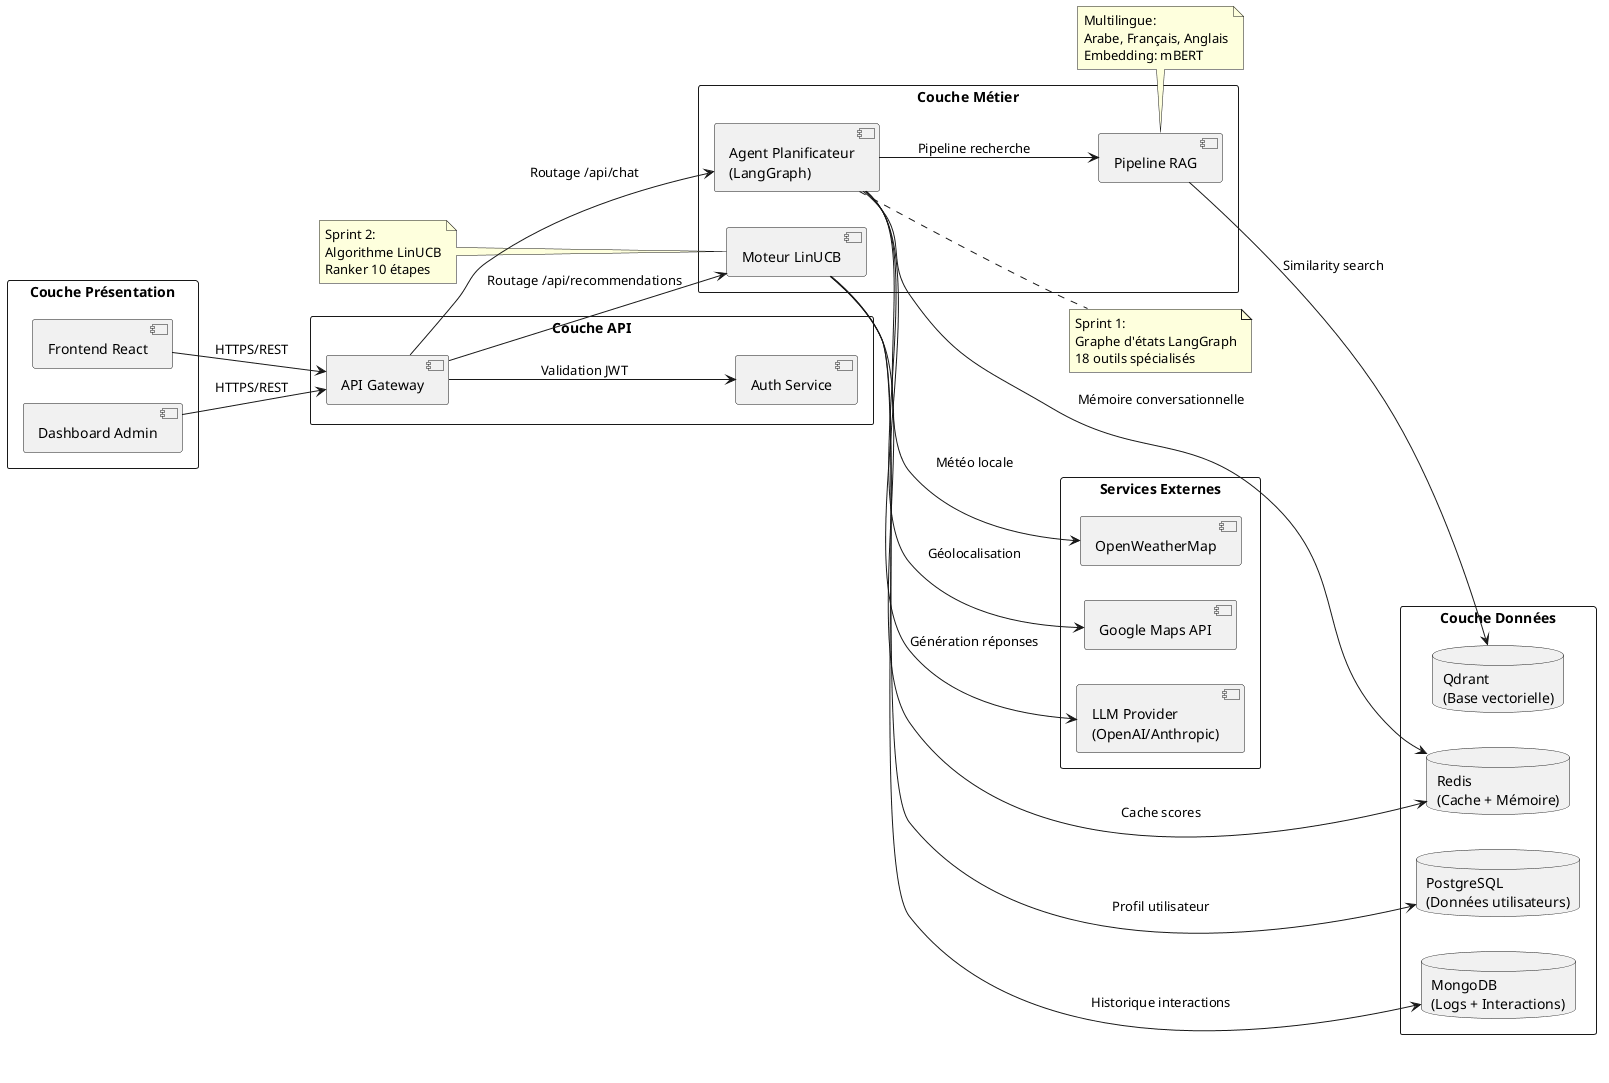
\includegraphics[width=\textwidth]{diagrams/plantuml/class_architecture.png}
    \caption{Architecture logique en couches du système Guidni}
    \label{fig:arch_logique}
\end{figure}

\subsection{Diagramme de cas d'utilisation global détaillé}

\begin{figure}[H]
    \centering
    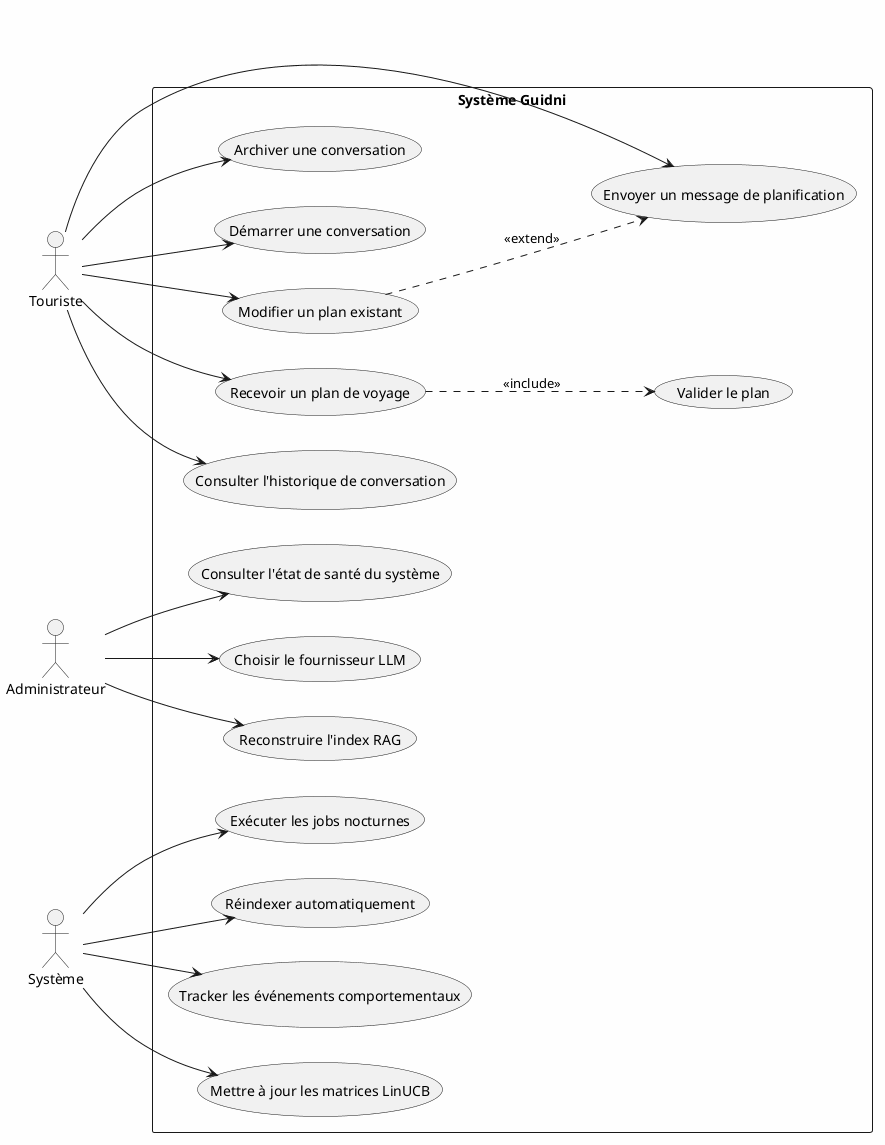
\includegraphics[width=\textwidth]{diagrams/fig_03_use_case_global.png}
    \caption{Diagramme de cas d'utilisation global détaillé}
    \label{fig:uc_global_detail}
\end{figure}

\subsection{Conception de la base de données}

Le backend IA lit 14~tables Prisma en lecture seule et possède en écriture 4~tables
planificateur et 7~tables recommandation.

\begin{figure}[H]
    \centering
    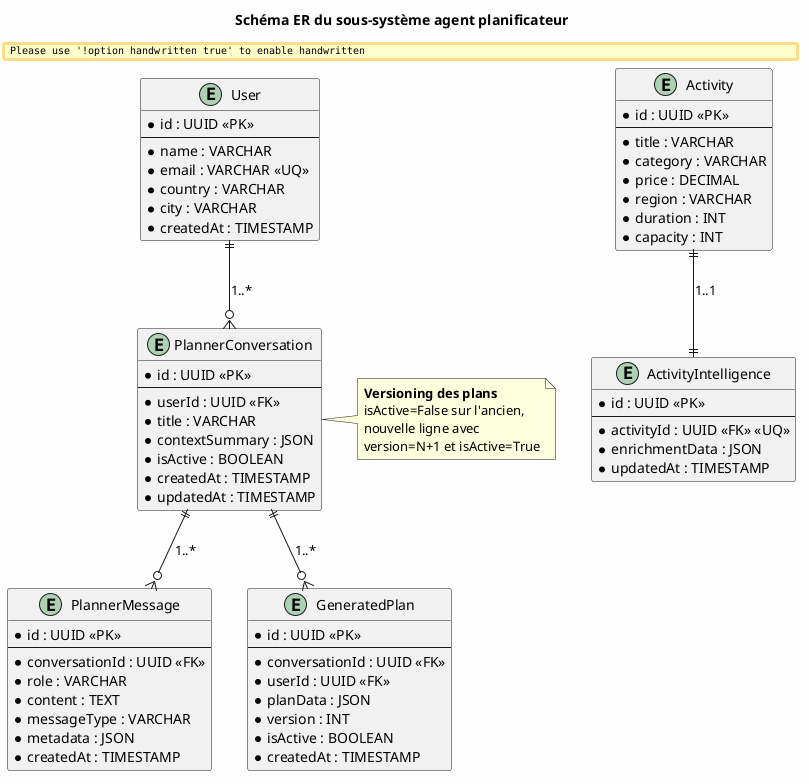
\includegraphics[width=\textwidth]{diagrams/fig_03_er_diagram_planner.png}
    \caption{Schéma ER du sous-système agent planificateur}
    \label{fig:er_planner}
\end{figure}

\begin{figure}[H]
    \centering
    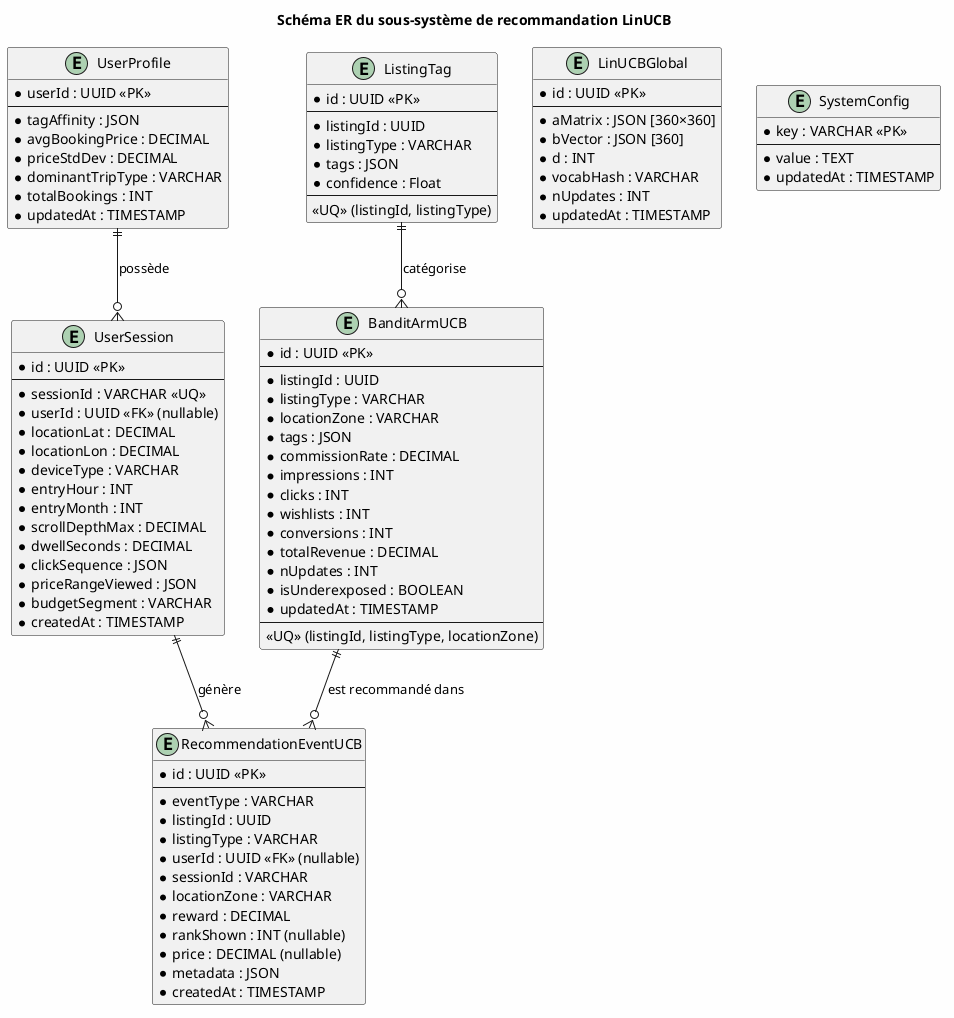
\includegraphics[width=\textwidth]{diagrams/fig_03_er_diagram_recommender.png}
    \caption{Schéma ER du sous-système de recommandation LinUCB}
    \label{fig:er_recommender}
\end{figure}


% ────────────────────────────────────────────────────────────────
\section{Product Backlog}
% ────────────────────────────────────────────────────────────────

Le Product Backlog recense l'ensemble des User Stories du projet, priorisées selon la méthode
MoSCoW (\textit{Must / Should / Could / Won't}).

\begin{table}[H]
    \centering
    \caption{Product Backlog du projet Guidni}
    \label{tab:product_backlog}
    \small
    \begin{tabular}{c p{9cm} c}
        \toprule
        \textbf{ID} & \textbf{User Story} & \textbf{Priorité} \\
        \midrule
        US-01 & En tant que touriste, je veux formuler des requêtes en langage naturel
        multilingue (FR/EN/AR) & Must \\[3pt]
        US-02 & En tant que touriste, je veux recevoir un itinéraire multi-jours personnalisé
        selon mon budget et mes préférences & Must \\[3pt]
        US-03 & En tant que touriste, je veux modifier mon plan par des messages de suivi & Must \\[3pt]
        US-04 & En tant que système, je veux effectuer des recherches sémantiques RAG dans le
        catalogue touristique & Must \\[3pt]
        US-05 & En tant que système, je veux intégrer les données météo en temps réel & Should \\[3pt]
        US-06 & En tant que système, je veux scorer les recommandations en $<$100\,ms grâce
        au cache matriciel LinUCB & Must \\[3pt]
        US-07 & En tant que touriste, je veux recevoir des recommandations adaptées à mon
        comportement de navigation & Must \\[3pt]
        US-08 & En tant que système, je veux collecter les signaux comportementaux du touriste
        via un tracker JavaScript & Must \\[3pt]
        US-09 & En tant qu'administrateur, je veux reconstruire l'index RAG & Should \\[3pt]
        US-10 & En tant que touriste, je veux consulter l'historique de mes conversations & Could \\[3pt]
        US-11 & En tant que système, je veux maintenir les profils utilisateurs via des jobs
        nocturnes & Should \\[3pt]
        US-12 & En tant que système, je veux vérifier l'intégrité du vocabulaire de tags par
        hachage SHA-256 & Must \\
        \bottomrule
    \end{tabular}
\end{table}


% ────────────────────────────────────────────────────────────────
\section{Planification des Sprints}
% ────────────────────────────────────────────────────────────────

Le tableau~\ref{tab:sprint_planning} présente la planification globale des quatre Sprints
du projet.

\begin{table}[H]
    \centering
    \caption{Planification des Sprints du projet Guidni}
    \label{tab:sprint_planning}
    \small
    \begin{tabular}{c c p{6.5cm} c}
        \toprule
        \textbf{Release} & \textbf{Sprint} & \textbf{Objectif} & \textbf{Période} \\
        \midrule
        \multirow{2}{*}{R1} & Sprint 1 & Mise en place de l'environnement, interface
        utilisateur et architecture de base & Oct. 2024 \\[3pt]
         & Sprint 2 & Implémentation du pipeline RAG multilingue et recherche sémantique &
        Nov. 2024 \\[3pt]
        \multirow{2}{*}{R2} & Sprint 3 & Agent LLM, machine à états LangGraph et planification
        conversationnelle & Déc. 2024 \\[3pt]
         & Sprint 4 & Moteur de recommandation LinUCB, tests et évaluation &
        Jan.--Fév. 2025 \\
        \bottomrule
    \end{tabular}
\end{table}

\begin{figure}[H]
    \centering
    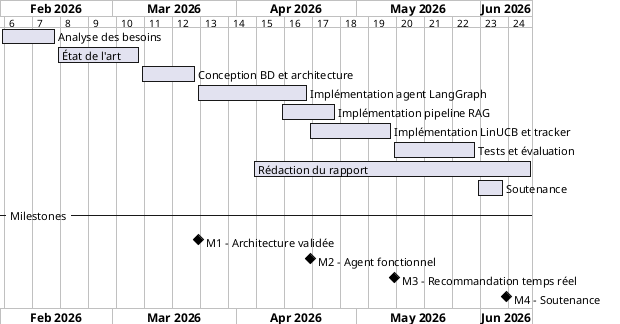
\includegraphics[width=\textwidth]{diagrams/fig_01_gantt.png}
    \caption{Diagramme de Gantt du projet Guidni}
    \label{fig:gantt}
\end{figure}


% ────────────────────────────────────────────────────────────────
\section{Environnement de travail et outils}
% ────────────────────────────────────────────────────────────────

\subsection{Environnement matériel}

Le développement a été effectué sur une machine locale dont les caractéristiques sont
présentées dans le tableau~\ref{tab:hardware}.

\begin{table}[H]
    \centering
    \caption{Caractéristiques de l'ordinateur de développement}
    \label{tab:hardware}
    \small
    \begin{tabular}{p{4cm} p{8cm}}
        \toprule
        \textbf{Composant} & \textbf{Spécification} \\
        \midrule
        Processeur & Multi-cœurs (x86\_64) \\[3pt]
        Mémoire vive & 16~Go DDR4 \\[3pt]
        Stockage & SSD NVMe \\[3pt]
        Système d'exploitation & Linux (Ubuntu) \\[3pt]
        GPU & Intégré (inférence CPU via Ollama) \\[3pt]
        Réseau & Fibre optique (tests API Cloud) \\
        \bottomrule
    \end{tabular}
\end{table}

\subsection{Environnement logiciel et outils}

\begin{table}[H]
    \centering
    \caption{Outils et technologies utilisés}
    \label{tab:outils}
    \small
    \begin{tabular}{p{3cm} p{4cm} p{5.5cm}}
        \toprule
        \textbf{Catégorie} & \textbf{Outil} & \textbf{Rôle} \\
        \midrule
        Langage backend & Python 3.12 & Logique agentique et moteur de recommandation \\[3pt]
        Framework API & FastAPI & API REST asynchrone (12 endpoints) \\[3pt]
        Orchestrateur IA & LangGraph / LangChain & Machine à états de l'agent \\[3pt]
        Index vectoriel & LlamaIndex & Pipeline RAG et stockage persistant \\[3pt]
        Embeddings & BAAI/bge-m3 & Projections multilingues (1024 dim.) \\[3pt]
        Reranker & BAAI/bge-reranker-v2-m3 & Cross-encoder de réordonnancement \\[3pt]
        Base de données & PostgreSQL 15 & Stockage relationnel partagé \\[3pt]
        ORM & SQLAlchemy (async) & Accès base de données côté IA \\[3pt]
        Frontend & Next.js / Prisma & Interface utilisateur et CRUD \\[3pt]
        LLM local & Ollama (qwen2.5:7b) & Inférence hors ligne \\[3pt]
        LLM cloud & Groq, Gemini, Lightning & Inférence rapide et contexte long \\[3pt]
        Planificateur & APScheduler & Jobs nocturnes de maintenance \\[3pt]
        Tests & pytest & Tests unitaires et d'intégration \\[3pt]
        IDE & VS Code & Environnement de développement \\[3pt]
        Versionnement & Git / GitHub & Gestion du code source \\
        \bottomrule
    \end{tabular}
\end{table}

Les figures suivantes présentent les logos des principales technologies utilisées dans le
projet Guidni. Chaque technologie a été choisie pour sa complémentarité avec les autres
composants du système.

\begin{figure}[H]
    \centering
    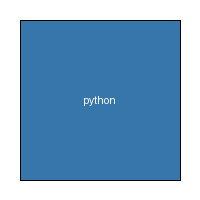
\includegraphics[width=0.12\textwidth]{logos/logo_python.png}
    \caption{Python 3.12 --- langage principal du backend IA, choisi pour son écosystème ML/NLP
    mature (LangChain, LlamaIndex, scikit-learn) et sa gestion asynchrone native via asyncio}
    \label{fig:logo_python}
\end{figure}

\begin{figure}[H]
    \centering
    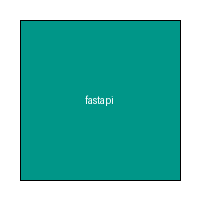
\includegraphics[width=0.12\textwidth]{logos/logo_fastapi.png}
    \caption{FastAPI --- framework web asynchrone haute performance basé sur Starlette et
    Pydantic, offrant une génération automatique de documentation OpenAPI et une validation
    de schémas par typage statique}
    \label{fig:logo_fastapi}
\end{figure}

\begin{figure}[H]
    \centering
    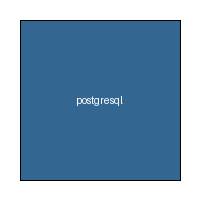
\includegraphics[width=0.12\textwidth]{logos/logo_postgresql.png}
    \caption{PostgreSQL 15 --- système de gestion de base de données relationnelle open source,
    choisi pour sa robustesse, son support de JSONB et son extension pgvector pour le stockage
    de vecteurs d'embeddings}
    \label{fig:logo_postgresql}
\end{figure}

\begin{figure}[H]
    \centering
    
\includegraphics[width=0.12\textwidth]{logos/logo_nextjs.png}
    \caption{Next.js --- framework React de production offrant le rendu côté serveur (SSR),
    le routage par fichiers et l'intégration native de Prisma ORM pour les opérations CRUD
    sur les entités touristiques}
    \label{fig:logo_nextjs}
\end{figure}

\begin{figure}[H]
    \centering
    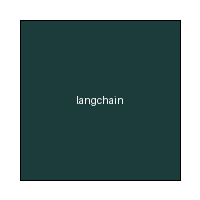
\includegraphics[width=0.12\textwidth]{logos/logo_langchain.png}
    \caption{LangGraph / LangChain --- framework d'orchestration agentique permettant de
    définir des machines à états typées avec routage conditionnel, mémoire persistante et
    appel d'outils structuré}
    \label{fig:logo_langchain}
\end{figure}

\begin{figure}[H]
    \centering
    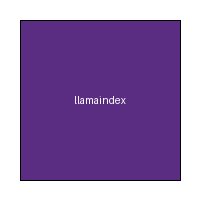
\includegraphics[width=0.12\textwidth]{logos/logo_llamaindex.png}
    \caption{LlamaIndex --- framework spécialisé dans l'indexation et la recherche sémantique,
    utilisé pour le pipeline RAG avec support de multiples moteurs vectoriels (pgvector, Qdrant)}
    \label{fig:logo_llamaindex}
\end{figure}

\begin{figure}[H]
    \centering
    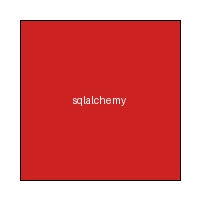
\includegraphics[width=0.12\textwidth]{logos/logo_sqlalchemy.png}
    \caption{SQLAlchemy --- ORM Python avec support asynchrone (asyncpg), utilisé pour l'accès
    aux données côté backend IA et pour les écouteurs d'événements de réindexation incrémentale}
    \label{fig:logo_sqlalchemy}
\end{figure}

\begin{figure}[H]
    \centering
    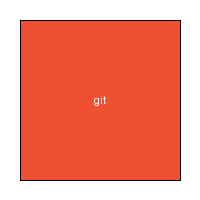
\includegraphics[width=0.12\textwidth]{logos/logo_git.png}
    \caption{Git / GitHub --- système de contrôle de version distribué utilisé pour la gestion
    du code source, le suivi des modifications et la collaboration}
    \label{fig:logo_git}
\end{figure}


% ────────────────────────────────────────────────────────────────
\section*{Conclusion}
\addcontentsline{toc}{section}{Conclusion}

Ce chapitre a permis de lancer formellement le projet Guidni. J'ai analysé les besoins
fonctionnels et non fonctionnels, défini les concepts théoriques fondamentaux (LLM, RAG,
LinUCB), conçu l'architecture globale du système, et établi le Product Backlog avec sa
priorisation MoSCoW. La planification en quatre Sprints a été présentée, couvrant l'ensemble
du cycle de développement d'octobre 2024 à février 2025. Enfin, l'environnement matériel
et logiciel a été détaillé avec les logos et descriptions des technologies retenues.

Le chapitre suivant détaillera le Sprint~1, consacré à la mise en place de l'environnement,
l'interface utilisateur et l'architecture de base du système.
